\chapter{数据库概念设计}

\section{确定实体和属性}
分析系统需求,将系统中设计的人、物进行抽象,得到了系统的实体如下:

\begin{enumerate}
    \item 论文:论文编号、论文标题、论文链接、摘要、发表日期
    \item 作者:作者编号、姓名、机构
    \item 代码:代码编号、代码链接、收藏数、框架
    \item 方法:方法编号、方法名、方法描述
    \item 评价指标:指标编号、得分计算方式
    \item 机器学习任务:任务编号、任务名称、任务描述
    \item 数据集:数据集编号、数据集名称、数据集描述、数据集链接、创建日期
\end{enumerate}

\section{E-R图}
系统E-R图见图 \ref{fig:er} 。

\begin{figure}[htbp!]
    \centering
    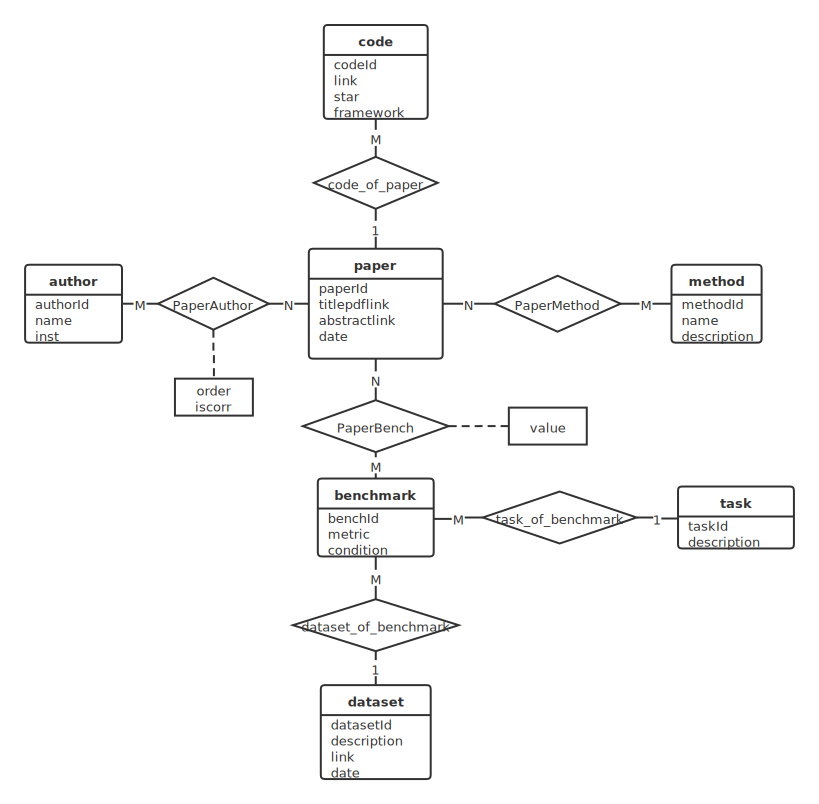
\includegraphics[width=\textwidth]{figures/Papers with Code.pdf}
    \caption{E-R图}
    \label{fig:er}
\end{figure}
